\documentclass[11pt,a4paper,roman]{moderncv}
\usepackage[english]{babel}
\usepackage[utf8]{inputenc}
\usepackage[T1]{fontenc}
\usepackage{lmodern}

% ModernCV themes
\moderncvstyle{classic}
\moderncvcolor{green}

\usepackage[scale=0.75]{geometry}
\usepackage{graphicx}
\usepackage{hyperref}

% Personal data
\name{Thanh}{Hoang-Minh}
\title{Application for Machine Learning Engineer Position}
\address{Ho Chi Minh City}{}{Vietnam}
\phone[mobile]{+84~913~472~506}
\email{hmthanhgm@gmail.com}
\homepage{hmthanh.github.io}

\begin{document}
	
	% Letter recipient
	\recipient{Motorica AI}{Hiring Team}
	\date{\today}
	\opening{Dear Motorica Team,}
	\closing{Thank you for your consideration. I look forward to the opportunity to discuss how I can contribute to Motorica's ongoing mission.}
	\enclosure[Attachment]{Curriculum Vitae}
	\makelettertitle
	
	With a solid foundation in machine learning and 3D motion animation, I believe I am well-suited for the \textbf{Machine Learning Engineer} position at \textbf{Motorica AI}.
	
	My proposed \textbf{DeepGesture} model - a transformer-diffusion hybrid designed to generate gestures from multimodal input (speech, emotion, and semantics) - demonstrates both research depth and engineering capability. I have also worked with the ZeroEGGS retargeting dataset (Daniel Holden) and developed the \href{https://github.com/DeepGesture/DeepGesture-Unity}{DeepGesture-Unity} project (AI4Animation - Sebastian Starke) to render gesture results directly within Unity.
	
	I'm also a co-organizer of the \textbf{GENEA Leaderboard} and \textbf{HEMVIP}, a system for evaluating multiple gesture generation models using Prolific. These efforts reflect my commitment to both academic rigor and scalable, production-focused systems.
	
	\begin{center}
		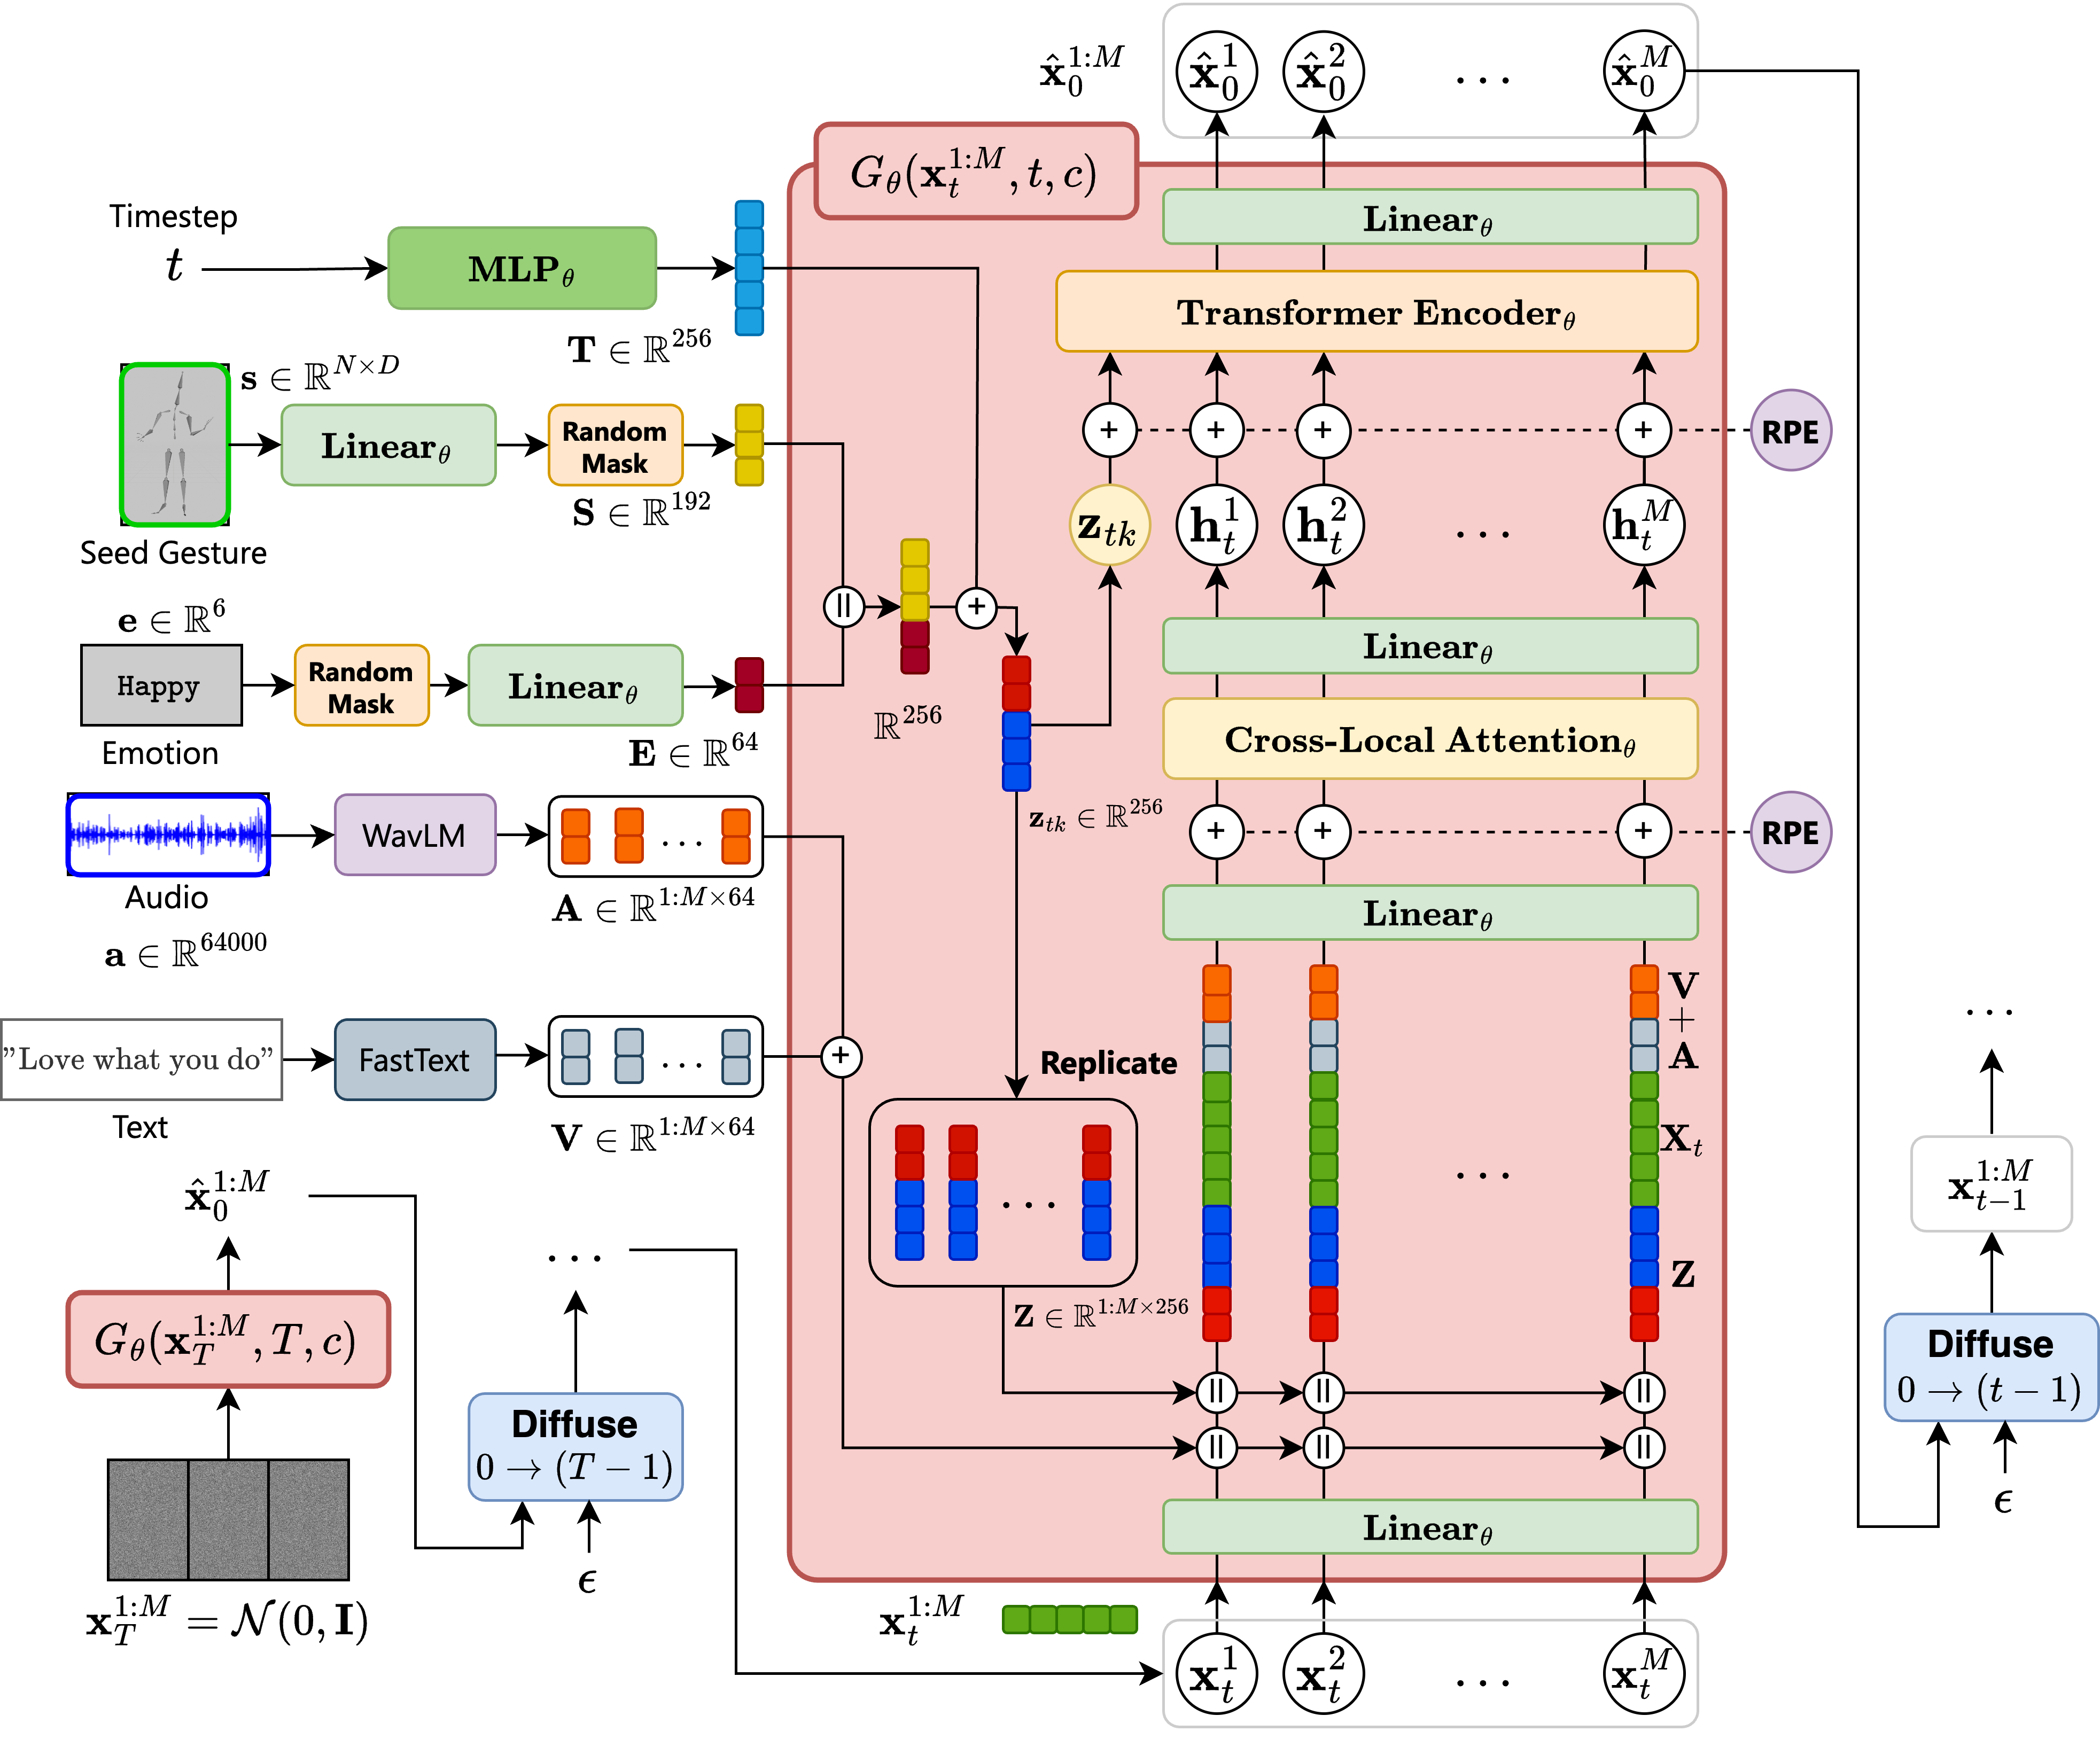
\includegraphics[width=0.8\linewidth]{DeepGesture.png} \\
		\small DeepGesture architecture. More details available at \href{https://deepgesture.github.io}{deepgesture.github.io}.
	\end{center}
	
	I am deeply passionate about digital humans and motion synthesis, with demonstrated skills in 3D rendering using Blender, including high-fidelity assets from 3DScanStore and Universal Human rendering scenes. I am particularly drawn to Motorica’s emphasis on foundational motion models and their integration with AAA game studios. My experience with skeleton retargeting using MotionBuilder, as well as building blendshape-based facial rigs, aligns well with Motorica’s production needs.
	
	Additionally, I have practical experience with Unity, demonstrated through my own game projects, and a strong foundation in 3D animation workflows. I am confident that this combination of skills positions me to contribute meaningfully to Motorica’s initiatives.
	
%	I would appreciate the opportunity to further discuss how my skill set, including diffusion model implementation, and 3D animation integration, and how can I directly support and accelerate Motorica’s research and production roadmap.
	
	\makeletterclosing
	
\end{document}
